\PassOptionsToPackage{svgnames}{xcolor}
\documentclass{book}
\usepackage[utf8]{inputenc}
\usepackage{graphicx}
\usepackage{listings}
\usepackage{hyperref}
\usepackage{amsmath}
\usepackage{xcolor}

\usepackage{tcolorbox}
\tcbuselibrary{skins,breakable}
\usetikzlibrary{shadings,shadows}

\newenvironment{myexampleblock}[1]{%
    \tcolorbox[beamer,%
    noparskip,breakable,
    colback=LightGreen,colframe=DarkGreen,%
    colbacklower=LimeGreen!75!LightGreen,%
    title={#1}, width=\textwidth]}%
    {\endtcolorbox}

\newenvironment{myalertblock}[1]{%
    \tcolorbox[beamer,%
    noparskip,breakable,
    colback=LightCoral,colframe=DarkRed,%
    colbacklower=Tomato!75!LightCoral,%
    title={#1}, width=\textwidth]}%
    {\endtcolorbox}

\newenvironment{myblock}[1]{%
    \tcolorbox[beamer,%
    noparskip,breakable,
    colback=LightBlue,colframe=DarkBlue,%
    colbacklower=DarkBlue!75!LightBlue,%
    title={#1}, width=\textwidth]}%
    {\endtcolorbox}

\newcommand{\code}[1]{\mbox{% added this percent
    \ttfamily
    \tcbox[
        on line,
        boxsep=0pt, left=4pt, right=4pt, top=2pt, bottom=1.5pt,
        toprule=0pt, rightrule=0pt, bottomrule=0pt, leftrule=0pt,
        oversize=0pt, enlarge left by=0pt, enlarge right by=0pt,
        colframe=white, colback=black!12,
        height=.8\baselineskip % added this (and guessed at .8)
    ]{#1}% added this percent
}}


\newtheorem{definition}{Definition}
\renewcommand{\chaptername}{Chapitre}

\begin{document}
\setlength{\parindent}{0cm}
\setcounter{chapter}{1}
\chapter{Outils de recherche}

Cette section de mon tutoriel porte sur des outils que j'ai trouvé utiles durant mes années d'études et de recherche. 


\section{Outils pour la recherche d'article}

Google Scholar \\
ArXiv \\
Zotero \\
ResearchRabbit

\section{Outils pour la rédaction}
LaTeX/Typst \\
Overleaf

\section{Outils pour le développement}
Deep learning frameworks : TensorFlow, PyTorch, Jax, Keras (Tuto 2 : PyTorch)\\
Machine learning important tools : Numpy, Pandas, Matplotlib/Seaborn/Plotly, Scikit-Learn (Tuto 3 : All things machine learning)\\
Experiment tracking : Wandb, MLflow \\
Google Colab/Jupyter Notebook, Kaggle \\
Hyperparameter tuning : Optuna, Ray Tune, Hyperopt

\section{LLMs}

Je recommande d’utiliser un LLM UNIQUEMENT SI vous pouvez vérifier l’output. 

Aussi, je recommande de ne jamais uploader du contenu sous copyright dans un LLM. J'ai demandé à Claude pour avoir une réponse dans la figure~\ref{fig:claude}.

\begin{figure}[!h]
    \centering
    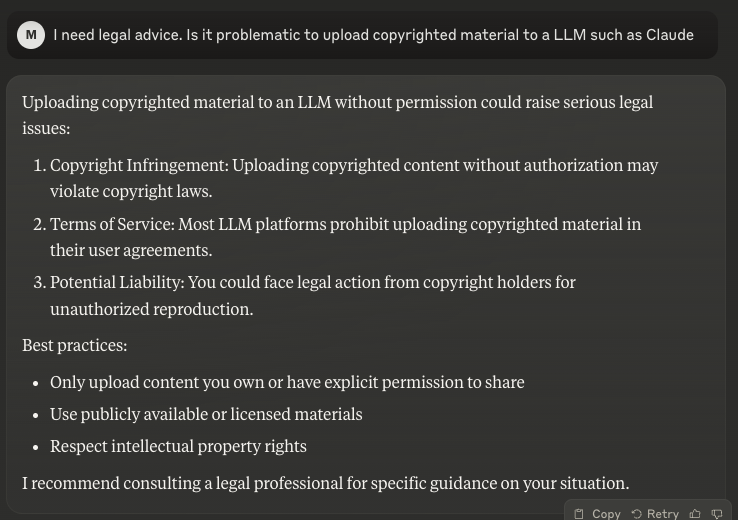
\includegraphics[width=\textwidth]{images/legal_claude.png}
    \caption{Réponse de Claude sur la question}\label{fig:claude}
\end{figure}

J'ai aussi trouvé très intéressant la phrase suivante, du \emph{Terms of Service} de ChatGPT. En effet, "[You may not] represent that Output was human-generated when it was not." \\

Finalement, même si les \emph{Terms of service} de ChatGPT indique que l'output est la propriété de l'utilisateur (voir figure~\ref{fig:chatgpt}), généralement le contenu généré par une IA n'est possédée par personne. Quoique ce n'est pas du tout une source scientifique, j'avais trouvé ce vidéo par un streamer assez intéressant : \url{https://youtu.be/pt7GtDMTd3k?si=MQNskBNIoZRPN70Z}.

\begin{figure}[!h]
    \centering
    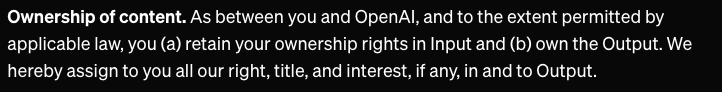
\includegraphics[width=\textwidth]{images/legal_chatgpt.png} 
    \caption{Propriété intellectuelle de la sortie d'une IA}\label{fig:chatgpt}
\end{figure}
LLMs disponibles : 

\textbf{ChatGPT} (toujours désactivé l’entraînement sur les données, paramètres section Gestion des données, désactivez "Améliorer le modèle pour tous") \\


\textbf{Claude} (selon leurs conditions d’utilisation, ils n’utilisent pas les données par défaut. Toutefois, ils ont quand même utilisés les donnés dans le papier de Clio (https://www.anthropic.com/research/clio) )\\

\textbf{Le chat} (Mistral) (ils disent que les données ne sont pas utilisées : https://help.mistral.ai/en/articles/156194-does-mistral-ai-exploit-users-data-to-train-its-models et que whatever données qui doivent être supprimées peuvent être fait en leur écrivant : https://help.mistral.ai/en/articles/154193-how-can-i-exercise-my-gdpr-rights)  \\

\textbf{Meta.ai} (il ne semble pas y avoir d’options pour la vie privée) \\

\textbf{DeepSeek} (selon ce post, c’est vraiment pas une bonne idée : https://medium.com/data-science-in-your-pocket/dont-use-deepseek-v3-895be7b853b0. ) 
You cannot use, copy, or even display any content or software from DeepSeek without permission.
Any misuse, even unintentional, may lead to legal action from DeepSeek. \\

 
\textbf{Gemini} (might not be able to opt out of data being used to train the model : https://www.googlecloudcommunity.com/gc/AI-ML/Use-of-your-data-for-product-improvement-purposes-in-the-Google/m-p/723832)  \\
\textbf{Copilot} (payé par l’université pour garantir la non-utilisation des données)\\


Avec un peu de volonté, il existe des modèles OpenSource qui peuvent être utilisés directement sur votre ordinateur. Par exemple, on a : 

\textbf{Lucie} : \url{https://huggingface.co/OpenLLM-France/Lucie-7B-Instruct}

\textbf{LLama} : \url{https://www.llama.com/docs/llama-everywhere/running-meta-llama-on-mac/}

Ça m'a pris environ 30 secondes à installer Ollama et je suis capable d'utiliser Lucie et Llama sans problème. L'environnement dans un terminal est moins bien, mais j'ai téléchargé oterm et ça semble fonctionner sans problème.
\section{Outils divers}
\url{https://github.com/yuchenlin/rebiber} \\
\url{https://github.com/google-research/arxiv-latex-cleaner}  \\
\url{https://capitalizemytitle.com/} \\
\url{https://flamingtempura.github.io/bibtex-tidy/index.html}  \\


\end{document}